\documentclass[12pt,a4paper]{article}
% Prefer pdfLaTeX if Cyrillic packages are installed.
% If pdfLaTeX fails because T2A Cyrillic support is missing, use LuaLaTeX instead.

\usepackage{iftex}
\ifPDFTeX
    \usepackage[utf8]{inputenc}
    \usepackage[T2A]{fontenc}
    \usepackage[bulgarian]{babel}
\else
    \usepackage{fontspec}
    \usepackage{polyglossia}
    \setdefaultlanguage{bulgarian}
    \setotherlanguage{english}
    \setmainfont{DejaVu Serif}
    \setsansfont{DejaVu Sans}
    \setmonofont{DejaVu Sans Mono}
\fi

\usepackage{geometry}
\usepackage{amsmath,amssymb}
\usepackage{graphicx}
\usepackage{booktabs}
\usepackage{float}
\usepackage{hyperref}
\usepackage{caption}
\usepackage{array}
\usepackage{makecell}
\usepackage{listings}
\usepackage{tikz}
\usetikzlibrary{arrows.meta,positioning,shapes.geometric}

\geometry{margin=2.5cm}
\graphicspath{{figures/}}
\hypersetup{
    colorlinks=true,
    linkcolor=black,
    urlcolor=blue,
    citecolor=black
}
\captionsetup{font=small}
\Urlmuskip=0mu plus 2mu
\lstdefinestyle{csmall}{
    language=C,
    basicstyle=\ttfamily\small,
    keywordstyle=\bfseries,
    commentstyle=\itshape,
    numbers=left,
    numberstyle=\tiny,
    stepnumber=1,
    numbersep=8pt,
    frame=single,
    showstringspaces=false,
    columns=fullflexible,
    keepspaces=true,
    xleftmargin=1em,
    framexleftmargin=1em,
    captionpos=b
}

\begin{document}

\hypersetup{pageanchor=false}
\begin{titlepage}
    \thispagestyle{plain}

    \noindent
    \begin{minipage}{0.17\textwidth}
        
\includegraphics[width=\linewidth]{3_TU_bg_n.png}
    \end{minipage}%
    \hspace{0.03\textwidth}%
    \begin{minipage}{0.8\textwidth}
        \raggedright
        \large
\textbf{ТЕХНИЧЕСКИ УНИВЕРСИТЕТ, СОФИЯ}\\[-0.3ex]
        \rule{\linewidth}{0.2pt}\\[-0.6ex]
        \textbf{ФАКУЛТЕТ КОМПЮТЪРНИ СИСТЕМИ И ТЕХНОЛОГИИ}\\[0.2cm]
    \end{minipage}

    \vspace{3cm}

    \begin{center}
        \textbf{\LARGE КУРСОВА РАБОТА}\\[1cm]

        \normalsize
        Дисциплина: Високопроизводителни компютърни системи\\[0.8cm]

        \textbf{Тема:}\\[0.3cm]
        \textbf{Сравнителен симулационен анализ на архитектури\\
        с последователно и извънредно изпълнение чрез gem5}\\[2.8cm]
    \end{center}

    \vspace{0.8cm}

    \begin{flushleft}
        \textbf{Изготвил:}\\
        Асен Пантелеев Попов\\
        Фак. № 121223246\\
        Група 38\\
        III курс, КСИ\\
        e-mail: \texttt{asepopov@tu-sofia.bg}
    \end{flushleft}

    \vspace{1.0cm}

    \begin{flushleft}
        \textbf{Ръководител:}\\
        доц. д-р инж. Ива Николова
    \end{flushleft}

    \vfill

    \begin{center}
        София, 2026 г.
    \end{center}
\end{titlepage}
\hypersetup{pageanchor=true}

\tableofcontents
\newpage

\section{Увод}
Съвременните високопроизводителни компютърни системи се стремят да повишават производителността не само чрез по-висока тактова честота, но и чрез по-ефективна микроархитектура. Един от основните архитектурни избори е дали инструкциите да се изпълняват строго в програмния ред или процесорът да може динамично да пренарежда изпълнението им. Този избор е особено важен при натоварвания, при които има разлика между изчислителна интензивност и латентност на паметта.

Настоящата курсова работа изследва чрез симулации в \texttt{gem5} поведението на две архитектури: \texttt{MinorCPU}, който реализира in-order изпълнение, и \texttt{O3CPU}, който реализира out-of-order изпълнение. Целта е да се анализира как архитектурният модел влияе върху IPC, CPI, общия брой цикли и кеш поведението при два типа натоварване: матрично умножение и pointer chasing.

\section{Цел на проекта}
Основната цел е да се извърши сравнителен анализ между in-order и out-of-order процесорна архитектура при еднакви системни условия. За да бъде сравнението коректно, и двете конфигурации използват една и съща ISA платформа, \texttt{X86}, еднаква честота от \texttt{3 GHz}, една и съща кеш йерархия с частни \texttt{L1I 32 KiB}, \texttt{L1D 32 KiB} и частен \texttt{L2 512 KiB}, както и една и съща памет \texttt{SingleChannelDDR3\_1600}. Следователно единствената променлива в експеримента е типът процесорно ядро, \texttt{MinorCPU} като in-order модел и \texttt{O3CPU} като out-of-order модел.

\section{Теоретична основа}

\subsection{Паралелизъм на ниво инструкции}
Паралелизмът на ниво инструкции (\emph{Instruction-Level Parallelism}, ILP) описва доколко различни инструкции могат да се изпълняват паралелно, без да нарушават коректността на програмата. Колкото повече независими инструкции има, толкова по-голям IPC може да постигне процесорът. Това е особено важно при изчислително-интензивни задачи, където има достатъчно операции, които могат да се подготвят и изпълняват едновременно.

\subsection{In-order изпълнение}
При in-order архитектурата инструкциите преминават през конвейера в реда, в който се срещат в програмата. Това опростява хардуера, но прави процесора по-чувствителен към stall-и. Когато дадена инструкция трябва да изчака резултат от паметта или от предходна зависимост, следващите инструкции също се забавят.

\subsection{Out-of-order изпълнение}
При out-of-order архитектурата процесорът може да избира готови за изпълнение инструкции, дори ако по-ранни инструкции все още чакат. Това се реализира чрез механизми като register renaming, instruction window, reorder buffer и dynamic scheduling. Благодарение на тях процесорът може да скрива част от латентността на паметта и да използва по-добре наличните изпълнителни блокове. Предимството е по-висок IPC, а недостатъкът е по-сложен и по-скъп за симулация и реализация хардуер.

\subsection{Метрики}
В анализа се използват следните основни метрики:

\begin{equation}
\text{IPC} = \frac{\text{Instructions}}{\text{Cycles}}
\end{equation}

\begin{equation}
\text{CPI} = \frac{\text{Cycles}}{\text{Instructions}}
\end{equation}

По-висок IPC и по-нисък CPI означават по-добро използване на процесора. Освен това се разглеждат:
общият брой цикли, L1D miss rate и L2 miss rate. Тези показатели позволяват едновременно да се оцени изчислителната ефективност и влиянието на паметната йерархия върху поведението на двата процесорни модела.

\subsection{Матрично умножение и невронни мрежи}
Матричното умножение е фундаментална операция не само в класическите числени алгоритми, но и в съвременните системи с изкуствен интелект. При плътно свързан невронен слой изходният вектор се изчислява като \(\mathbf{a}=\phi(W\mathbf{x}+\mathbf{b})\), където \(W\) е матрица от тегла, \(\mathbf{x}\) е входен вектор, \(\mathbf{b}\) е bias вектор, а \(\phi\) е активационна функция. При обработка на множество наблюдения едновременно същата операция естествено се формулира като матрично умножение. Поради това производителността на операции от типа GEMM е пряко свързана с ефективността на inference и training натоварвания в невронните мрежи \cite{aimet}. На практика значителна част от изчислителното натоварване при линейни слоеве, attention механизми и convolution lowering техники се свежда именно до такива матрични операции. Това означава, че наблюденията върху поведението на матричното умножение в рамките на настоящата работа имат пряка връзка с по-широк клас реални AI изчисления. В контекста на проекта benchmark-ът за матрично умножение е подходящ не само като типично изчислително-интензивно натоварване, но и като опростен представител на реални приложения.

\begin{figure}[H]
    \centering
    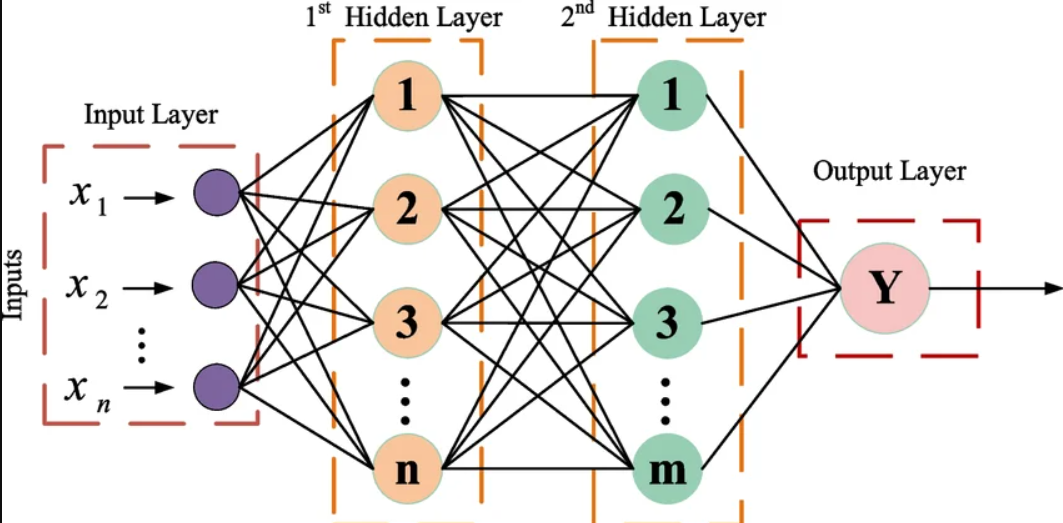
\includegraphics[width=0.74\textwidth]{MLP.png}
    \caption{Примерна структура на multilayer perceptron, при която връзките между слоевете се реализират чрез матрични операции \cite{mlpsoftsensor}.}
\end{figure}

\begin{figure}[H]
    \centering
    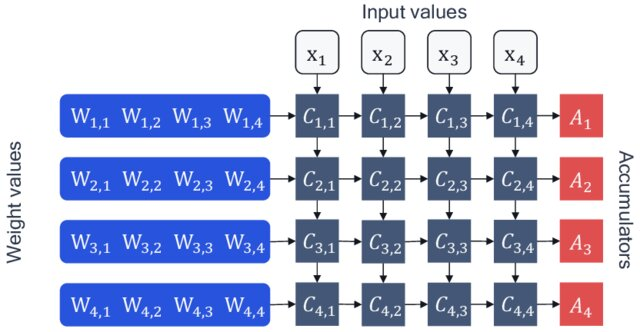
\includegraphics[width=0.82\textwidth]{Matrix_Multiplication.png}
    \caption{Илюстрация на ролята на матричното умножение при изчисляването на изходите на невронен слой \cite{aimet}.}
\end{figure}

\section{Методология на експеримента}

\subsection{Симулационна среда}
Експериментите са изпълнени със симулатора \texttt{gem5}, компилиран като \texttt{build/X86/gem5.opt}. Използван е syscall-emulation режим, който позволява директно изпълнение на локални \texttt{X86} Linux бинарни файлове без пълна операционна система в симулацията. Този подход е достатъчен за целите на задачата, тъй като изследователският въпрос е фокусиран върху микроархитектурната разлика между \texttt{MinorCPU} и \texttt{O3CPU}, а не върху full-system поведение.

\begin{figure}[H]
    \centering
    \begin{tikzpicture}[
        node distance=0.9cm and 0.5cm,
        procbox/.style={draw, rounded corners, minimum width=2.6cm, minimum height=0.9cm, align=center, font=\small},
        arrow/.style={-{Latex[length=2.5mm]}, thick}
    ]
        \node[procbox] (src) {C benchmark-и};
        \node[procbox, right=of src] (bin) {X86 бинарни\\файлове};
        \node[procbox, right=of bin] (cfg) {gem5 конфигурация\\(\texttt{run\_se.py})};
        \node[procbox, below=of cfg, xshift=-1.6cm] (minor) {\texttt{MinorCPU}};
        \node[procbox, below=of cfg, xshift=1.6cm] (o3) {\texttt{O3CPU}};
        \node[procbox, below=of minor, xshift=1.6cm] (stats) {\texttt{stats.txt}};
        \node[procbox, left=of stats] (csv) {\texttt{summary.csv}};
        \node[procbox, left=of csv] (plots) {Таблици и\\графики};

        \draw[arrow] (src) -- (bin);
        \draw[arrow] (bin) -- (cfg);
        \draw[arrow] (cfg) -- (minor);
        \draw[arrow] (cfg) -- (o3);
        \draw[arrow] (minor) -- (stats);
        \draw[arrow] (o3) -- (stats);
        \draw[arrow] (stats) -- (csv);
        \draw[arrow] (csv) -- (plots);
    \end{tikzpicture}
    \caption{Работен поток на експеримента от benchmark-ите до крайните резултати.}
\end{figure}

\subsection{Конфигурация на системата}
И за двата CPU модела е използвана една и съща системна конфигурация: едно ядро върху \texttt{X86Board}, тактова честота \texttt{3 GHz}, кеш йерархия с \texttt{L1I 32 KiB}, \texttt{L1D 32 KiB} и частен \texttt{L2 512 KiB}, както и \texttt{SingleChannelDDR3\_1600} с \texttt{3 GiB} симулирана памет. Този избор гарантира, че отчетените разлики се дължат на микроархитектурния модел, а не на различна паметна или кеш конфигурация.

\begin{table}[H]
    \centering
    \small
    \setlength{\tabcolsep}{6pt}
    \begin{tabular}{l l}
        \toprule
        Параметър & Стойност \\
        \midrule
        ISA / платформа & \texttt{X86Board} \\
        Режим на симулация & syscall emulation (SE) \\
        Брой ядра & 1 \\
        Честота & \texttt{3 GHz} \\
        L1 instruction cache & \texttt{32 KiB} \\
        L1 data cache & \texttt{32 KiB} \\
        L2 cache & \texttt{512 KiB} \\
        Основна памет & \texttt{SingleChannelDDR3\_1600} \\
        Симулирана памет & \texttt{3 GiB} \\
        Сравнявана променлива & \texttt{MinorCPU} срещу \texttt{O3CPU} \\
        Натоварвания & \texttt{matrix\_multiply}, \texttt{pointer\_chase} \\
        \bottomrule
    \end{tabular}
    \caption{Фиксирани параметри на експерименталната конфигурация}
\end{table}

\subsection{Използвани натоварвания}
Използвани са два benchmark-а, създадени специално за проекта. Те представляват два различни режима на поведение: изчислително-интензивно натоварване с добра локалност и натоварване, ограничено от латентността на паметта и от зависимите адресации.

\paragraph{Матрично умножение.}
Това натоварване изпълнява класически тройно вложен цикъл за умножение на матрици. Характеризира се с добра локалност на данните и с висока изчислителна интензивност. Подобен тип операция е в основата и на плътните слоеве в невронните мрежи, поради което benchmark-ът има и приложна стойност извън чисто числения пример. Очакването е out-of-order архитектурата да извлече повече ILP и да постигне значително по-висок IPC.

\begin{lstlisting}[style=csmall,caption={Откъс от benchmark-а за матрично умножение},label={lst:matrix}]
for (long i = 0; i < n; ++i) {
    for (long j = 0; j < n; ++j) {
        int64_t sum = 0;

        for (long k = 0; k < n; ++k) {
            sum += (int64_t)a[(size_t)i * (size_t)n + (size_t)k] *
                   (int64_t)bt[(size_t)j * (size_t)n + (size_t)k];
        }

        c[(size_t)i * (size_t)n + (size_t)j] = (int32_t)sum;
    }
}
\end{lstlisting}

Кодът показва класическия тройно вложен цикъл, при който във вътрешния цикъл се извършват многократни операции умножение и натрупване. Това създава благоприятни условия за използване на ILP и за ефективно натоварване на изпълнителните блокове.

\paragraph{Pointer chasing.}
Това натоварване изгражда псевдослучайна свързана структура в масив и след това обхожда елементите чрез последователност от зависими индиректни адресации. Характеризира се с ниска локалност и със силна зависимост между стъпките, което ограничава ILP и увеличава вероятността от cache misses. Очакването е предимството на \texttt{O3CPU} да бъде осезаемо по-малко, тъй като дори агресивното пренареждане на инструкции не може да скрие напълно зависимите латентности на паметта.

\begin{lstlisting}[style=csmall,caption={Откъс от benchmark-а за pointer chasing},label={lst:pointer}]
for (long i = 0; i < nodes; ++i) {
    long next_i = (i + 1) % nodes;
    next[order[i]] = order[next_i];
}

index = order[0];

for (uint64_t step = 0; step < (uint64_t)nodes * (uint64_t)steps_per_node;
     ++step) {
    index = next[index];
    checksum += (uint64_t)index;
}
\end{lstlisting}

Тук всяка следваща адресация зависи от стойността, заредена в предходната стъпка. Именно тази зависимост прави натоварването чувствително към латентността на паметта и силно ограничава възможностите за пренареждане на инструкции.

\subsection{Събрани статистики}
От \texttt{stats.txt} за всяко изпълнение са извлечени \texttt{simInsts}, \texttt{numCycles}, \texttt{ipc}, \texttt{cpi}, \texttt{l1d miss rate} и \texttt{l2 miss rate}. Тъй като броят симулирани инструкции е еднакъв в рамките на всяка двойка сравнявани натоварвания, метриките за цикли, IPC и CPI могат да бъдат използвани директно за коректна оценка на производителността.

\subsection{Валидност на сравнението}
Сравнението между двата процесорни модела е конструирано така, че да изолира единствено ефекта от микроархитектурата. За всяка двойка експерименти натоварването, ISA платформата, кеш конфигурацията, паметната система и честотата са еднакви. Освен това броят симулирани инструкции е идентичен в рамките на всяка двойка: при матричното умножение и двата модела изпълняват \(29\,077\,226\) инструкции, а при pointer chasing и двата модела изпълняват \(12\,431\,387\) инструкции. Следователно разликите в IPC, CPI и общия брой цикли могат да бъдат интерпретирани като реален ефект от in-order спрямо out-of-order изпълнение, а не като следствие от различна програма или различна системна конфигурация.

\section{Реализация}
За проекта беше изградена автоматизирана експериментална рамка. Създадени бяха два локални benchmark-а на \texttt{C}, shell скрипт за компилация на бинарните файлове, конфигурационен Python скрипт за \texttt{gem5} и автоматизиран launcher за четирите експеримента: \texttt{matrix\_minor}, \texttt{matrix\_o3}, \texttt{pointer\_minor} и \texttt{pointer\_o3}. Резултатите бяха обобщени автоматично в \texttt{summary.csv}, а върху тях бяха генерирани таблици и графики за отчета. По този начин целият експериментален процес, от компилацията до извличането на метриките, беше възпроизводим и еднакъв за всички конфигурации.

\subsection{Публично хранилище на проекта}
Кодът на проекта е публикуван в GitHub хранилище \cite{projectrepo}: \url{https://github.com/Apsie09/Gem5-Microarchitecture-Analysis}. В него са включени benchmark програмите на \texttt{C}, конфигурационният код за \texttt{gem5}, shell и Python скриптовете за изпълнение на експериментите и извличане на статистиките, генерираните обобщени резултати, както и \LaTeX{} изходният код на настоящия отчет в директорията \texttt{report}. Това позволява експериментите и документацията да бъдат проследени, проверени и повторени независимо.

\section{Резултати}

\subsection{Основна сравнителна таблица}
\begin{table}[H]
    \centering
    \small
    \setlength{\tabcolsep}{5pt}
    \begin{tabular}{l l r r r r r r}
        \toprule
        Натоварване & CPU & \makecell[r]{Инструкции\\(M)} & \makecell[r]{Цикли\\(M)} & IPC & CPI & \makecell[r]{L1D\\miss rate} & \makecell[r]{L2\\miss rate} \\
        \midrule
        Matrix & Minor & 29.08 & 65.32 & 0.445 & 2.246 & 0.000869 & 0.015299 \\
        Matrix & O3 & 29.08 & 11.05 & 2.631 & 0.380 & 0.003427 & 0.015169 \\
        Pointer & Minor & 12.43 & 159.69 & 0.078 & 12.845 & 0.357979 & 0.463546 \\
        Pointer & O3 & 12.43 & 112.25 & 0.111 & 9.030 & 0.372311 & 0.477100 \\
        \bottomrule
    \end{tabular}
    \caption{Сравнение между \texttt{MinorCPU} и \texttt{O3CPU} при двата типа натоварване}
\end{table}

Таблицата показва ясно, че за матричното умножение \texttt{O3CPU} постига драстично по-висока ефективност от \texttt{MinorCPU}, докато при pointer chasing предимството остава, но е по-умерено. По този начин още на таблично ниво се вижда разликата между compute-bound и memory-bound поведение.

\subsection{Производни показатели}
\begin{table}[H]
    \centering
    \small
    \setlength{\tabcolsep}{6pt}
    \begin{tabular}{l r r r}
        \toprule
        Натоварване & \makecell[r]{IPC\\speedup} & \makecell[r]{Намаление\\на CPI} & \makecell[r]{Намаление\\на циклите} \\
        \midrule
        Matrix & \(5.91\times\) & \(83.08\%\) & \(83.08\%\) \\
        Pointer & \(1.42\times\) & \(29.70\%\) & \(29.71\%\) \\
        \bottomrule
    \end{tabular}
    \caption{Обобщени производни показатели за \texttt{O3CPU} спрямо \texttt{MinorCPU}}
\end{table}

Тази таблица концентрира основния резултат на проекта в кратка форма. При матричното умножение out-of-order моделът носи много голямо ускорение, докато при pointer chasing подобрението е осезаемо, но ограничено от зависимостите между адресациите и от по-високата чувствителност към латентността на паметта.

\subsection{Графичен анализ}
Графиките потвърждават изводите от табличния анализ и позволяват по-бързо визуално сравнение между двата модела. Най-ясно се откроява, че при матричното умножение разликата между \texttt{MinorCPU} и \texttt{O3CPU} е значително по-голяма, отколкото при pointer chasing, докато кеш miss rate показва, че по-високата производителност на \texttt{O3CPU} не произтича непременно от по-добра локалност, а от по-ефективно използване на наличния ILP и по-добро скриване на латентността.

\begin{figure}[H]
    \centering
    \begin{minipage}{0.48\textwidth}
        \centering
        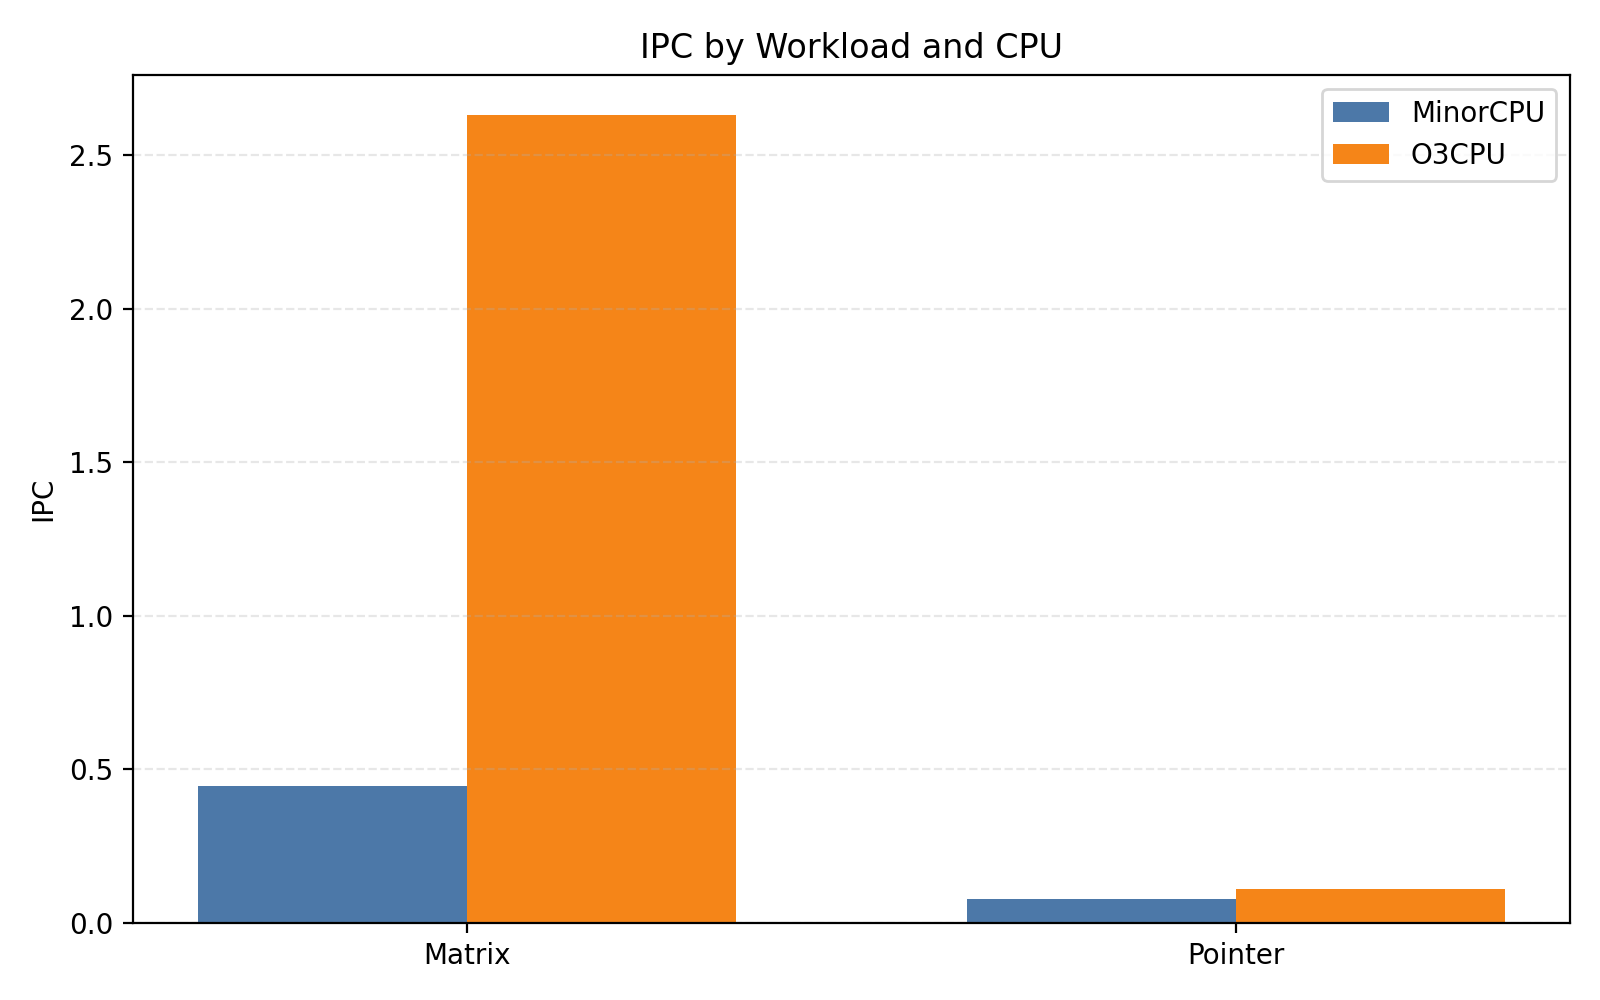
\includegraphics[width=\linewidth]{ipc.png}
        \caption{IPC по натоварване и тип процесор.}
    \end{minipage}\hfill
    \begin{minipage}{0.48\textwidth}
        \centering
        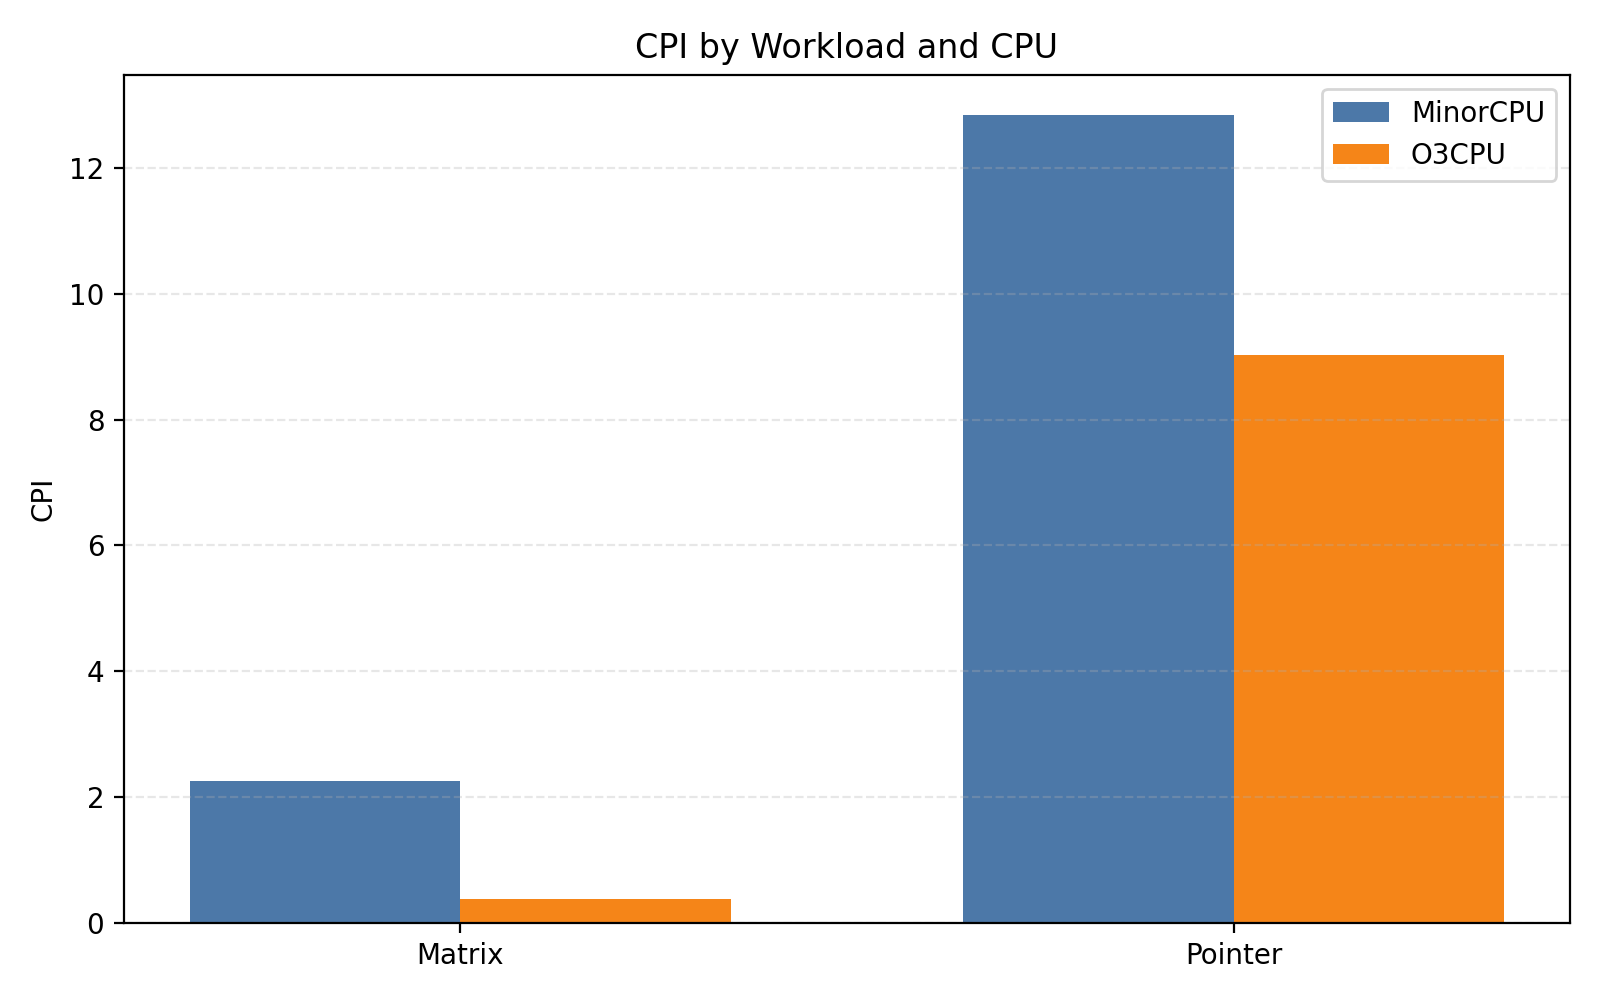
\includegraphics[width=\linewidth]{cpi.png}
        \caption{CPI по натоварване и тип процесор.}
    \end{minipage}
\end{figure}

\begin{figure}[H]
    \centering
    \begin{minipage}{0.48\textwidth}
        \centering
        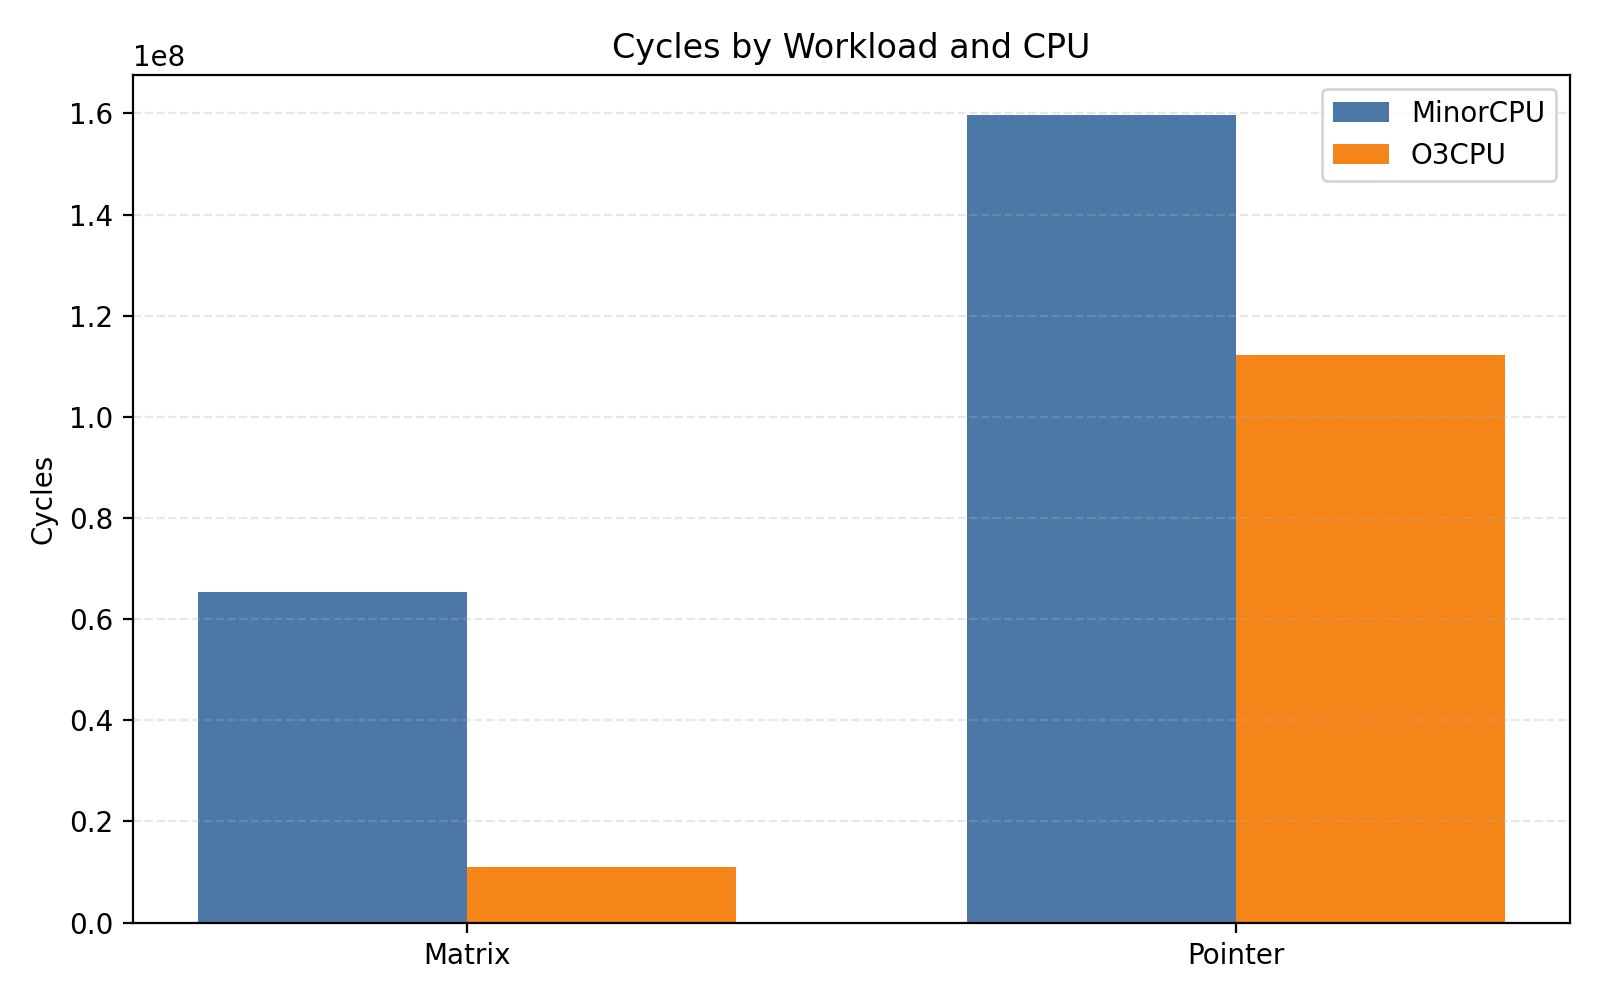
\includegraphics[width=\linewidth]{num_cycles.png}
        \caption{Общ брой цикли по натоварване и тип процесор.}
    \end{minipage}\hfill
    \begin{minipage}{0.48\textwidth}
        \centering
        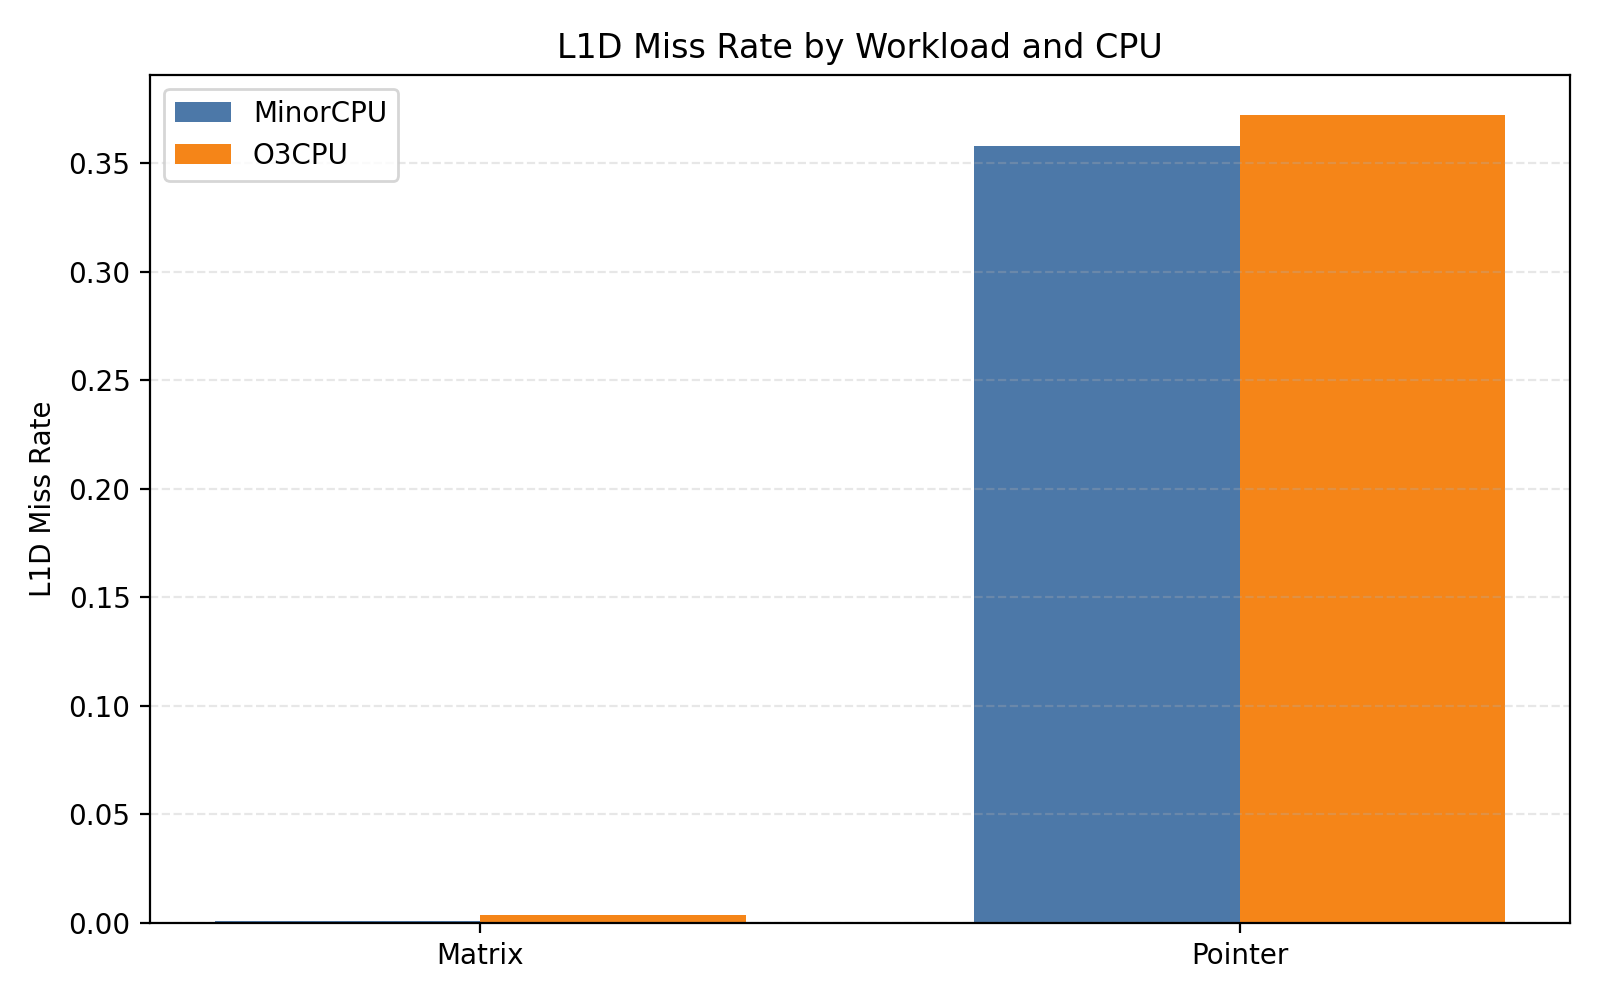
\includegraphics[width=\linewidth]{l1d_miss_rate.png}
        \caption{L1D miss rate по натоварване и тип процесор.}
    \end{minipage}
\end{figure}

\begin{figure}[H]
    \centering
    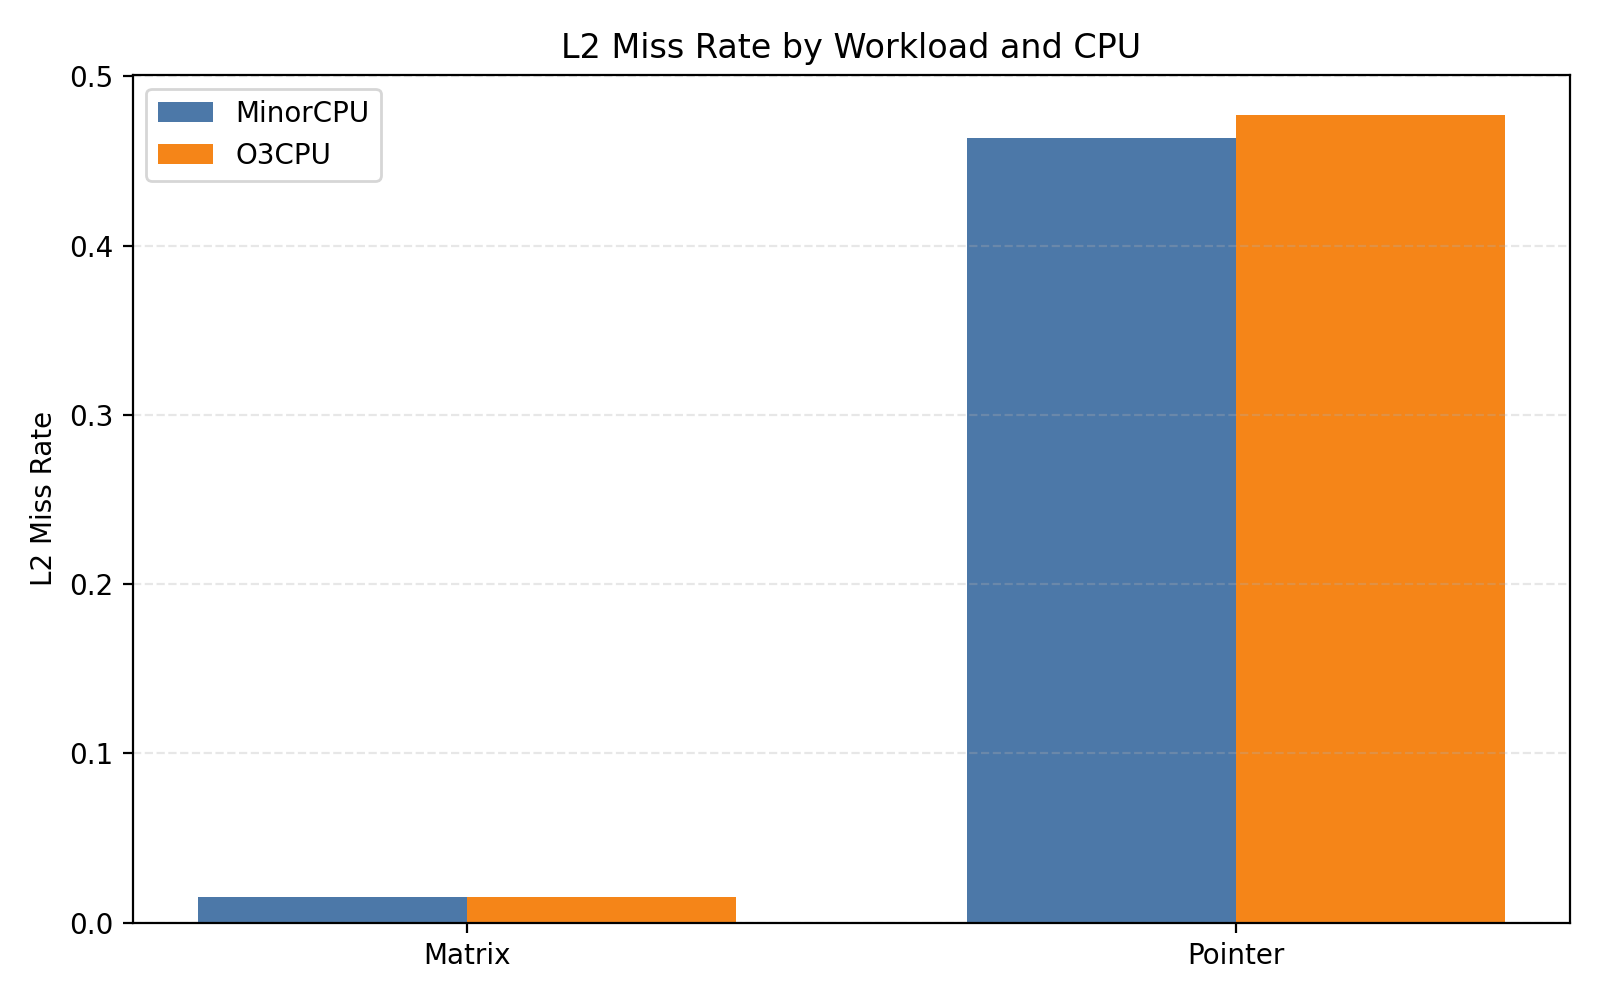
\includegraphics[width=0.56\textwidth]{l2_miss_rate.png}
    \caption{L2 miss rate по натоварване и тип процесор.}
\end{figure}

Визуално представяне на графиките показва, че IPC и броят цикли реагират много по-силно на промяната в микроархитектурата при compute-bound натоварването, отколкото при memory-bound натоварването. От друга страна, L1D и L2 miss rate остават високи при pointer chasing и за двата процесорни модела, което подкрепя извода, че тук ограничението идва основно от паметната система.

\subsection{Количествени изводи}
За матричното умножение \texttt{O3CPU} постига приблизително \(5.91\times\) по-висок IPC спрямо \texttt{MinorCPU}. Едновременно с това CPI намалява с около \(83.1\%\), а общият брой цикли също намалява с приблизително \(83.1\%\). Това е силно изразено предимство на out-of-order архитектурата при compute-bound натоварване.

За pointer chasing \texttt{O3CPU} постига само около \(1.42\times\) по-висок IPC. CPI намалява с приблизително \(29.7\%\), а общият брой цикли намалява с приблизително \(29.7\%\). Предимството е реално, но е значително по-малко, което е очаквано при memory-bound задача.

\section{Обсъждане}
Получените резултати потвърждават основната хипотеза на проекта и показват ясно, че ефектът от out-of-order изпълнението зависи от характера на натоварването. При матричното умножение разликата между \texttt{MinorCPU} и \texttt{O3CPU} е много голяма, тъй като натоварването има добра локалност и съдържа достатъчно независими операции. Това позволява на \texttt{O3CPU} да използва по-ефективно изпълнителните блокове и да повиши значително IPC, като едновременно с това намали CPI и общия брой цикли.

При pointer chasing ситуацията е качествено различна. Тук всяка следваща адресация зависи от резултата от предходната, което силно ограничава ILP. Освен това и при двата CPU модела L1D и L2 miss rate остават високи. Следователно доминиращият фактор е латентността на паметта, а не способността на процесора да пренарежда независими инструкции. В такава среда \texttt{O3CPU} продължава да има предимство, но то е значително по-малко, отколкото при матричното умножение.

Особено показателен е фактът, че \texttt{O3CPU} не постига непременно по-нисък miss rate. При матричния benchmark стойността на L1D miss rate за \texttt{O3CPU} дори е малко по-висока от тази за \texttt{MinorCPU}, но въпреки това \texttt{O3CPU} е многократно по-бърз по отношение на симулираните цикли и IPC. Това показва, че основното предимство на out-of-order изпълнението не е задължително подобряване на локалността, а по-ефективно скриване на латентността и по-добро използване на готовите за изпълнение инструкции.

Следва да се разграничават и две различни понятия за производителност: симулираната производителност на моделируемия процесор и реалното време за изпълнение на симулацията върху хост машината. Например при pointer chasing \texttt{O3CPU} е по-добър по симулирани цикли, но изисква повече host време. Това не е противоречие, а естествен резултат от факта, че \texttt{O3CPU} е по-сложен микроархитектурен модел и съответно е по-скъп за симулация.

\section{Ограничения и бъдеща работа}
Настоящият експеримент използва само два benchmark-а и едноядрена конфигурация. Това е достатъчно за ясен първоначален сравнителен анализ, но не покрива всички възможни класове натоварвания. Освен това е използван syscall-emulation режим, а не full-system симулация. Този избор е оправдан с оглед на поставената задача, но изключва влиянието на операционната система, прекъсванията и по-сложните многопрограмни сценарии.

Като естествено продължение на работата могат да се разгледат по-голям набор от benchmark-и, вариране на кеш размери и латентности, сравнение при други ISA платформи и многoядрени конфигурации. Полезно направление е и включването на допълнителни натоварвания, свързани с линейна алгебра и AI inference, така че връзката между микроархитектурния модел и реалните приложения да бъде анализирана още по-непосредствено. Практически ценно разширение би било и по-тясното интегриране на автоматичното извличане на статистики с LaTeX workflow, така че таблиците и графиките да се обновяват автоматично при всяко ново изпълнение на експериментите.

\section{Заключение}
В настоящата курсова работа беше реализиран и изпълнен сравнителен симулационен анализ на \texttt{MinorCPU} и \texttt{O3CPU} чрез \texttt{gem5}. При еднакви кеш, памет и честота беше показано, че out-of-order архитектурата носи голямо предимство при изчислително-интензивно натоварване и по-ограничено, но все пак осезаемо предимство при натоварване, доминирано от латентността на паметта.

Най-силно изразеният резултат е при матричното умножение, където \texttt{O3CPU} постига приблизително \(5.9\times\) по-висок IPC и около \(83\%\) по-малко цикли. При pointer chasing предимството остава, но е значително по-слабо: приблизително \(1.42\times\) по-висок IPC и около \(30\%\) по-малко цикли. Следователно основният извод е, че ефектът от out-of-order изпълнението зависи силно от характера на натоварването и е най-голям тогава, когато съществува достатъчен ILP и когато паметната латентност не е доминиращият ограничител.

\addcontentsline{toc}{section}{Литература}
\begin{thebibliography}{99}

\bibitem{gem5}
The gem5 Developers.
\newblock gem5 Documentation.
\newblock Available at: \url{https://www.gem5.org/documentation/}

\bibitem{hennessy}
Hennessy, J. L., Patterson, D. A.
\newblock \emph{Computer Architecture: A Quantitative Approach}.
\newblock Morgan Kaufmann.

\bibitem{minor}
The gem5 Developers.
\newblock Minor CPU Model Documentation.
\newblock Available at: \url{https://www.gem5.org/documentation/general_docs/cpu_models/minor_cpu}

\bibitem{o3}
The gem5 Developers.
\newblock O3CPU Model Documentation.
\newblock Available at: \url{https://www.gem5.org/documentation/general_docs/cpu_models/O3CPU}

\bibitem{aimet}
S. Siddegowda, M. Fournarakis, M. Nagel, T. Blankevoort, C. Patel, A. Khobare.
\newblock Neural Network Quantization with AI Model Efficiency Toolkit.
\newblock arXiv:2201.08442, 2022.

\bibitem{mlpsoftsensor}
L. Zhang, B. Wang, Y. Shen, Y. Nie.
\newblock An online soft sensor method for biochemical reaction process based on JS-ISSA-XGBoost.
\newblock \emph{BMC Biotechnology}, 23:49, 2023.
\newblock Available at: \url{https://doi.org/10.1186/s12896-023-00816-3}

\bibitem{projectrepo}
A. Popov.
\newblock Gem5 Microarchitecture Analysis.
\newblock GitHub repository.
\newblock Available at: \url{https://github.com/Apsie09/Gem5-Microarchitecture-Analysis}

\end{thebibliography}

\end{document}
